\documentclass[10pt,a4paper]{article}

\usepackage[margin=1.5cm,top=1.2cm,bottom=1.2cm]{geometry}
\usepackage[T1]{fontenc}
\usepackage[utf8]{inputenc}
\usepackage{mathptmx}
\usepackage{amsmath,amssymb}
\usepackage{booktabs}
\usepackage{array}
\usepackage{enumitem}
\usepackage{xcolor}
\usepackage{fancyhdr}
\usepackage[nobottomtitles*]{titlesec}
\renewcommand{\bottomtitlespace}{0.04\textheight}
\titlespacing*{\section}{0pt}{7pt}{3pt}
\titleformat*{\section}{\normalsize\bfseries\color{navy}}
\usepackage[colorlinks=true,linkcolor=black,urlcolor=blue!60!black]{hyperref}
\usepackage{graphicx}
\usepackage{wrapfig}
\usepackage{tikz}
\usetikzlibrary{positioning,arrows.meta}
\usepackage{listings}
\lstset{language=Python, basicstyle=\ttfamily\footnotesize, columns=fullflexible, keepspaces=true,
        commentstyle=\color{gray!70!black}, keywordstyle=\color{navy}, frame=single,
        rulecolor=\color{gray!40}, xleftmargin=4pt, xrightmargin=4pt, aboveskip=4pt, belowskip=2pt}

% ---------- Report information (edit here) ----------
\newcommand{\myname}{Arnab Kumar Ghosh}
\newcommand{\reporttitle}{Progress Report}
\newcommand{\projecttitle}{Discrete State-Space Models and Expectation-Maximization for Cell-State Trajectories}
\newcommand{\supervisor}{Prashant Singh}
\newcommand{\period}{Weeks 5--6}
\newcommand{\reportdate}{\today}
% ----------------------------------------------------

\definecolor{navy}{RGB}{31,56,100}
\setlist{nosep, leftmargin=1.4em}
\setlength{\parskip}{2pt}
\AtBeginDocument{\setlength{\abovedisplayskip}{4pt}\setlength{\belowdisplayskip}{4pt}}
\setlength{\parindent}{0pt}

\pagestyle{fancy}
\fancyhf{}
\rhead{\small Progress report -- \period}
\cfoot{\small\thepage}
\renewcommand{\headrulewidth}{0.3pt}

\newcommand{\sub}[1]{\vspace{1pt}\textbf{\textcolor{gray!80!black}{#1}}\par}

\begin{document}

% ---------- Title block ----------
\begin{center}
  {\Large\bfseries\textcolor{navy}{\reporttitle}}\\[2pt]
  {\projecttitle}\\[3pt]
  {\small \myname\ \textperiodcentered\ Supervisor: \supervisor\ \textperiodcentered\ MSc Computer Science, Uppsala University \textperiodcentered\ \period\ \textperiodcentered\ \reportdate}
\end{center}
\vspace{-2pt}
\hrule
\vspace{4pt}

% ---------- 0. Overview ----------
\section*{Overview}
The main open question of the last report was how to build the observation sequence. In the meeting on 6 October the supervisor and I worked through the population-level model on the whiteboard. In weeks 5--6 I wrote this model down as a likelihood, with its E-step and M-step (Sections 1--4), the starting values (Section 5), what the data can and cannot determine (Section 6), and a plan to test it on a toy example (Section 7). Figure~\ref{fig:flow} summarises the model and the fitting procedure. Progress against the plan from the last report:

\begin{enumerate}
  \item Bilmes (1998) and Gaussian emissions in the toy code: \textbf{started} implementing the toy example of the population model (Section 7).
  \item Write down the population-level likelihood, E-step and M-step with the supervisor: \textbf{done} (Sections 1--4).
  \item Open \texttt{adata\_final.h5ad}, check the normalisation, compute state proportions per time point: \textbf{started} looking at the data; I contacted the previous student for an overview of it.
  \item Read Amoedo-Leite et al.\ (2024): \textbf{started} reading.
  \item Validation set-up: \textbf{written down} (Section 6), not yet implemented.
\end{enumerate}

% ---------- 1 ----------
\section{The population-level model}

\sub{What I learned}
Sequencing destroys the cell, so each cell is measured once and no cell can be followed over time. A standard HMM needs one system observed again and again, so no sequence of individual cells can be built. What the data do support is the proportion of cells in each state on each day. The model therefore follows the population, not single cells. Let $p_t = (p_t[\mathrm{MA}], p_t[\mathrm{T}], p_t[\mathrm{MU}])$ be the state proportions in week $t$. They are linked by one transition matrix:
\[
p_{t+1} = p_t \cdot A, \qquad p_0 = \pi, \qquad \text{so} \qquad p_t = \pi \cdot A^t .
\]
Written out: $p_1 = p_0 A = \pi A$, $p_2 = p_1 A = \pi A^2$, $p_3 = p_2 A = \pi A^3$. Each week adds one factor of $A$, so the power of $A$ equals the number of weeks since day 0. One step is one week: $t = 0, 1, 2, 3$ for day 0, 7, 14 and 21. The same $A$ is used for every week. $p_t$ is a row vector.

$A[i,j]$ is now the fraction of the state-$i$ population that is in state $j$ one week later, not the path of one cell. The off-diagonal entries give the direction and the speed of reprogramming. $\pi$ is learned, not fixed. Most cells should start as macrophages, so $\pi$ should come out close to $(1,0,0)$, but not exactly.

\sub{In the project}
This replaces the sequence $O = o_1\, o_2\, o_3$ (day 7, 14, 21) of the last report. Day 0 is the healthy tissue, before injury, so the healthy cells enter the model as the first time point. Section 6 shows why this time point is needed.

\begin{figure}[!htb]
\centering
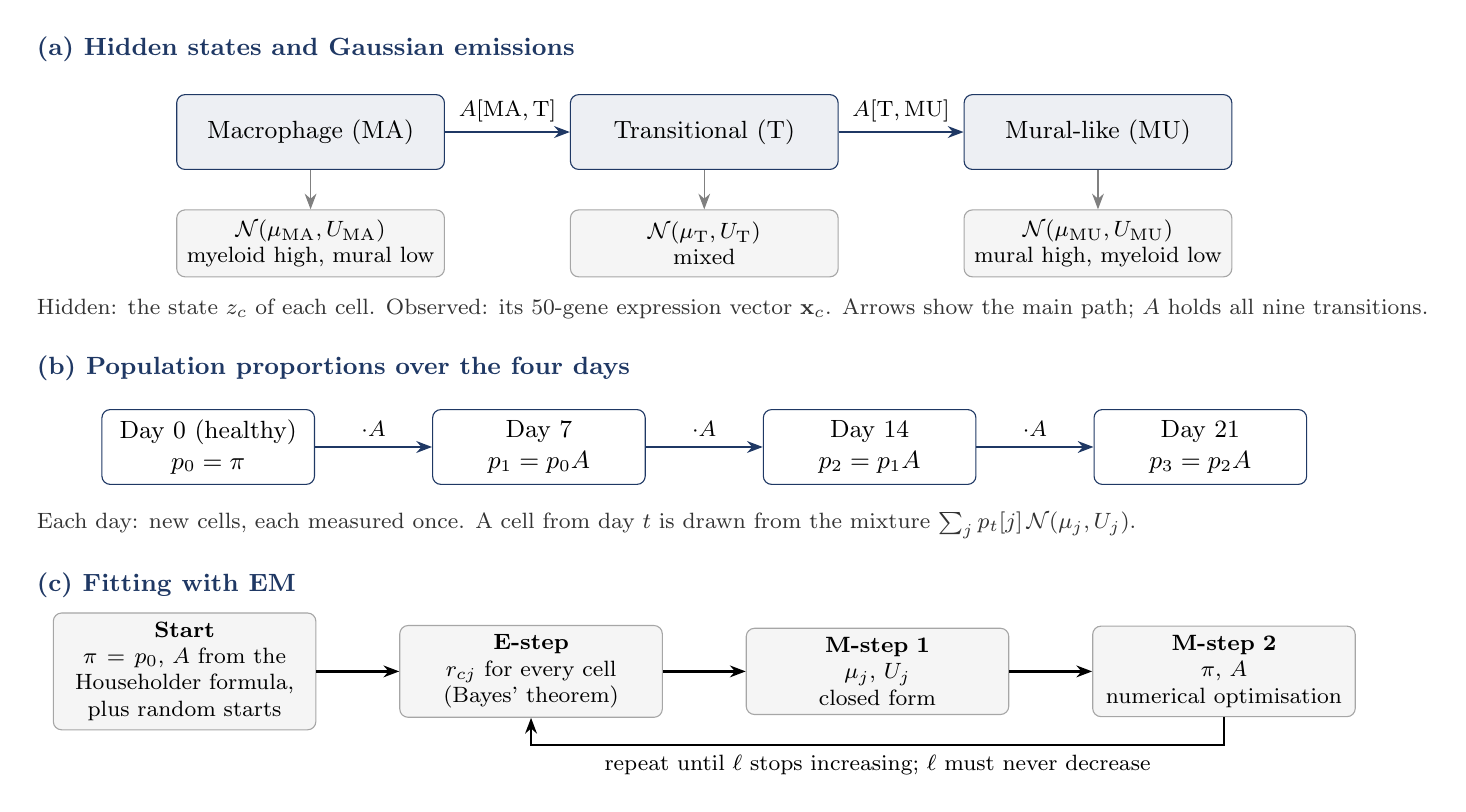
\begin{tikzpicture}[
  font=\small,
  >={Stealth[length=2mm]},
  state/.style={draw=navy, fill=navy!8, rounded corners=3pt, minimum width=3.4cm, minimum height=0.95cm, align=center},
  emit/.style={draw=gray!70, fill=gray!8, rounded corners=3pt, minimum width=3.4cm, minimum height=0.85cm, align=center, font=\footnotesize},
  day/.style={draw=navy, fill=white, rounded corners=3pt, minimum width=2.7cm, minimum height=0.95cm, align=center},
  emstep/.style={draw=gray!70, fill=gray!8, rounded corners=3pt, minimum height=1.0cm, align=center, font=\footnotesize, text width=3.1cm},
  panel/.style={font=\small\bfseries, text=navy, anchor=west},
  lab/.style={font=\footnotesize, midway, above}
]
% (a) hidden states and Gaussian emissions
\node[panel] at (-8.6,1.05) {(a) Hidden states and Gaussian emissions};
\node[state] (ma) at (-5,0) {Macrophage (MA)};
\node[state] (tr) at (0,0) {Transitional (T)};
\node[state] (mu) at (5,0) {Mural-like (MU)};
\draw[->, thick, navy] (ma) -- node[lab, text=black]{$A[\mathrm{MA},\mathrm{T}]$} (tr);
\draw[->, thick, navy] (tr) -- node[lab, text=black]{$A[\mathrm{T},\mathrm{MU}]$} (mu);
\node[emit, below=0.5cm of ma] (ema) {$\mathcal{N}(\mu_{\mathrm{MA}}, U_{\mathrm{MA}})$\\ myeloid high, mural low};
\node[emit, below=0.5cm of tr] (etr) {$\mathcal{N}(\mu_{\mathrm{T}}, U_{\mathrm{T}})$\\ mixed};
\node[emit, below=0.5cm of mu] (emu) {$\mathcal{N}(\mu_{\mathrm{MU}}, U_{\mathrm{MU}})$\\ mural high, myeloid low};
\draw[->, gray] (ma) -- (ema);
\draw[->, gray] (tr) -- (etr);
\draw[->, gray] (mu) -- (emu);
\node[font=\footnotesize, text=gray!40!black, anchor=west] at (-8.6,-2.25) {Hidden: the state $z_c$ of each cell. Observed: its 50-gene expression vector $\mathbf{x}_c$. Arrows show the main path; $A$ holds all nine transitions.};

% (b) population proportions over the four days
\node[panel] at (-8.6,-3.0) {(b) Population proportions over the four days};
\node[day] (d0) at (-6.3,-4.0) {Day 0 (healthy)\\ $p_0 = \pi$};
\node[day] (d1) at (-2.1,-4.0) {Day 7\\ $p_1 = p_0 A$};
\node[day] (d2) at (2.1,-4.0) {Day 14\\ $p_2 = p_1 A$};
\node[day] (d3) at (6.3,-4.0) {Day 21\\ $p_3 = p_2 A$};
\draw[->, thick, navy] (d0) -- node[lab, text=black]{$\cdot A$} (d1);
\draw[->, thick, navy] (d1) -- node[lab, text=black]{$\cdot A$} (d2);
\draw[->, thick, navy] (d2) -- node[lab, text=black]{$\cdot A$} (d3);
\node[font=\footnotesize, text=gray!40!black, anchor=west] at (-8.6,-5.0) {Each day: new cells, each measured once. A cell from day $t$ is drawn from the mixture $\sum_j p_t[j]\,\mathcal{N}(\mu_j, U_j)$.};

% (c) fitting with EM
\node[panel] at (-8.6,-5.75) {(c) Fitting with EM};
\node[emstep] (s0) at (-6.6,-6.85) {\textbf{Start}\\ $\pi = p_0$, $A$ from the Householder formula, plus random starts};
\node[emstep] (s1) at (-2.2,-6.85) {\textbf{E-step}\\ $r_{cj}$ for every cell\\ (Bayes' theorem)};
\node[emstep] (s2) at (2.2,-6.85) {\textbf{M-step 1}\\ $\mu_j$, $U_j$\\ closed form};
\node[emstep] (s3) at (6.6,-6.85) {\textbf{M-step 2}\\ $\pi$, $A$\\ numerical optimisation};
\draw[->, thick] (s0) -- (s1);
\draw[->, thick] (s1) -- (s2);
\draw[->, thick] (s2) -- (s3);
\draw[->, thick] (s3.south) -- ++(0,-0.35) -| node[pos=0.25, below, font=\footnotesize]{repeat until $\ell$ stops increasing; $\ell$ must never decrease} (s1.south);
\end{tikzpicture}
\caption{(a) Three hidden states, each with one Gaussian over the expression vector, shared across all days. (b) No cell is followed over time; the state proportions of the population move from week to week by one transition matrix $A$. (c) EM fits $\pi$, $A$, $\mu$ and $U$ together.}
\label{fig:flow}
\end{figure}

% ---------- 2 ----------
\section{Gaussian emissions}

\sub{What I learned}
Each state $j$ has one Gaussian over the expression vector $\mathbf{x}_c$ of a cell, shared across all days. Here $z_c$ is the hidden state of cell $c$, and $d$ is the number of genes:
\[
\mathbf{x}_c \mid z_c = j \;\sim\; \mathcal{N}(\mu_j, U_j), \qquad U_j = \mathrm{diag}(\sigma^2_{j,1}, \ldots, \sigma^2_{j,d}).
\]
$\mathcal{N}(\mu_j, U_j)$ is the multivariate normal (Gaussian) distribution with mean vector $\mu_j$ and covariance matrix $U_j$:
\begin{itemize}
  \item Mean vector: $\mu_j = (\mu_{j,1}, \ldots, \mu_{j,d})$ holds the typical expression of each gene in state $j$.
  \item Covariance matrix: $U_j$ is a $d \times d$ matrix. Its diagonal entry $\sigma^2_{j,g}$ is the variance of gene $g$ in state $j$. Its off-diagonal entry $(g, h)$ is the covariance of genes $g$ and $h$, i.e.\ how much they rise and fall together within the state.
  \item Diagonal covariance: I set all off-diagonal entries to zero. Within a state, the genes are then treated as independent, and only the $d$ variances are learned.
\end{itemize}
The formula has no $t$ in it: the same three Gaussians are used on every day, and only the mixture weights change. With a diagonal $U_j$ the density is a product of one-gene densities, so its log is a sum over the genes:
\[
\log \mathcal{N}(\mathbf{x}_c; \mu_j, U_j) = \sum_{g=1}^{d} \Big[ -\tfrac12 \log(2\pi\sigma^2_{j,g}) - \frac{(x_{c,g} - \mu_{j,g})^2}{2\sigma^2_{j,g}} \Big].
\]
The formula comes from three steps:
\begin{itemize}
  \item One gene: the density of gene $g$ in state $j$ is the 1D Gaussian $\frac{1}{\sqrt{2\pi\sigma^2_{j,g}}} \exp\!\big(-\frac{(x_{c,g}-\mu_{j,g})^2}{2\sigma^2_{j,g}}\big)$.
  \item Log: the fraction becomes the size term $-\tfrac12 \log(2\pi\sigma^2_{j,g})$, and the exponential leaves the distance term $-\frac{(x_{c,g}-\mu_{j,g})^2}{2\sigma^2_{j,g}}$.
  \item All genes: with a diagonal $U_j$ the genes are independent within a state, so the density of the cell is a product over genes, and its log is a sum over genes.
\end{itemize}
The distance term compares the value of gene $g$ in the cell, $x_{c,g}$, with the typical value of that gene in state $j$, $\mu_{j,g}$. The difference is squared and divided by the variance, so it is measured relative to how much the gene normally varies in that state. If the value is close to the mean, the term is close to zero. The further the value is from the mean, the more negative the term becomes, and the less the cell fits state $j$. The size term depends only on the spread: a wider Gaussian has a lower peak. The sum adds the evidence of all $d$ genes.

Two reasons for this form. Diagonal: a full $50 \times 50$ covariance has $50 \times 50 = 2500$ entries, but it is symmetric: the covariance of genes $g$ and $h$ equals that of $h$ and $g$, so every off-diagonal number appears twice. The free numbers are the 50 variances on the diagonal plus $(2500 - 50)/2 = 1225$ covariances, in total $d(d+1)/2 = 1275$ per state. A diagonal covariance sets all covariances to zero and keeps only the 50 variances. Log form: multiplying 50 small densities underflows to zero, adding 50 logs does not.

\sub{In the project}
$d = 50$: the top 25 marker genes of cluster 2 and of cluster 8. I will use log-normalised values.

% ---------- 3 ----------
\section{Likelihood and E-step}

\sub{What I learned}
A cell measured in week $t$ comes from a mixture of the three Gaussians, with the weights $p_t$ of that week. Given the parameters $\lambda = (\pi, A, \mu, U)$, the cells are independent, so the log-likelihood is a sum over cells:
\[
\ell(\lambda) = \sum_{c} \log \sum_{j=1}^{3} p_{t_c}[j]\, \mathcal{N}(\mathbf{x}_c; \mu_j, U_j).
\]
The weights of the four days are not free: they all come from one $\pi$ and one $A$. This is the time coupling. Without it, the model would be four unrelated mixture models. The inner sum is computed with log-sum-exp, a way to add the terms in log space without underflow.

The E-step is Bayes' theorem for each cell. The prior is the proportion of the cell's week, and the likelihood is the Gaussian density:
\[
r_{cj} = \frac{p_{t_c}[j]\, \mathcal{N}(\mathbf{x}_c; \mu_j, U_j)}{\sum_{k} p_{t_c}[k]\, \mathcal{N}(\mathbf{x}_c; \mu_k, U_k)} .
\]
$r_{cj}$ plays the role of $\gamma_t(i)$, but no forward--backward pass is needed. The day matters: the same expression vector can get different $r$ on different days, because the prior $p_{t_c}$ differs from week to week.

\textbf{Computed in five steps.} The denominator of $r_{cj}$ and the inner sum of $\ell$ are the same number, so it is computed once. With 50 genes every $\mathcal{N}$ can round to zero, so all steps are done in logs (a product becomes a sum, a division becomes a difference):
\begin{enumerate}[label=\arabic*.]
  \item Prior of the cell's week: $p_{t_c} = \pi A^{t_c}$.
  \item Log of the numerator of $r_{cj}$: \quad $a_{cj} = \log p_{t_c}[j] + \log \mathcal{N}(\mathbf{x}_c; \mu_j, U_j)$.
  \item Log of the denominator (log-sum-exp): \quad $\ell_c = \log \sum_k e^{a_{ck}} = m_c + \log \sum_k e^{a_{ck} - m_c}$, \quad $m_c = \max_k a_{ck}$.
  \item Numerator divided by denominator: \quad $r_{cj} = e^{a_{cj} - \ell_c}$.
  \item Log-likelihood: \quad $\ell = \sum_c \ell_c$.
\end{enumerate}
Subtracting the largest term $m_c$ in step 3 makes the largest exponential exactly $e^0 = 1$, so the sum cannot round to zero. Each step is one line of code (\texttt{population.py}); the comments carry the step numbers:
\begin{lstlisting}
# Step 1. Prior of each cell = proportions of its own week: (n, N)
proportions = get_proportions(pi, A, NUMBER_OF_WEEKS)   # (W, N), row t is p_t
priors = proportions[weeks]                              # row c is p_{t_c}
# Step 2. a_cj = log p_{t_c}[j] + log N(x_c; mu_j, U_j): (n, N)
log_densities = log_gaussian_densities(X, means, variances)
log_weights = np.log(priors) + log_densities
# Step 3. l_c = log sum_k exp(a_ck): (n,)
row_logsumexp = logsumexp(log_weights, axis=1)
# Step 4. r_cj = exp(a_cj - l_c): (n, N)
r = np.exp(log_weights - row_logsumexp[:, np.newaxis])
# Step 5. l = sum_c l_c
log_likelihood = np.sum(row_logsumexp)
\end{lstlisting}
\texttt{proportions[weeks]} picks row $t$ of the proportions once for every cell measured in week $t$, so each cell gets the prior of its own week. Worked example, hand-check cell $\mathbf{x} = (3, 2)$ from week 1 (toy model of Section 7):

\begin{center}
\small
\begin{tabular}{@{}llrrr@{}}
\toprule
Step & Quantity & MA & T & MU \\
\midrule
1 & $p_1[j]$ & 0.7260 & 0.1665 & 0.1075 \\
  & $\log \mathcal{N}(\mathbf{x}; \mu_j, I)$ (Section 2) & $-2.8379$ & $-2.0879$ & $-5.8379$ \\
2 & $a_j = \log p_1[j] + \log \mathcal{N}$ & $-3.1581$ & $-3.8806$ & $-8.0681$ \\
3 & $\ell_c = \log(e^{-3.1581} + e^{-3.8806} + e^{-8.0681})$ & \multicolumn{3}{c}{$-2.7574$} \\
4 & $r_j = e^{a_j - \ell_c}$ & 0.6698 & 0.3252 & 0.0049 \\
\midrule
  & check without logs: $p_1[j]\,\mathcal{N}$ & 0.0425 & 0.0206 & 0.0003 \\
\bottomrule
\end{tabular}
\end{center}
Without logs, the three numerators add up to $0.0635$; dividing each by this sum gives the same $r$, and $\log 0.0635 = -2.7574 = \ell_c$. The code reproduces these values and the total $\ell = -12.0361$ of the four hand-check cells.

\sub{In the project}
Each cell gets three state probabilities. The existing labels (\texttt{cell\_type}, \texttt{cluster}) are used only as an outside check of these probabilities, never as training input.

% ---------- 4 ----------
\newpage
\section{M-step}

\sub{What I learned}
\textbf{Gaussians (closed form):} For every state $j$ and gene $g$, summing over all cells of all days:
\[
\mu_{j,g} = \frac{\sum_c r_{cj}\, x_{c,g}}{\sum_c r_{cj}}, \qquad
\sigma^2_{j,g} = \frac{\sum_c r_{cj}\, (x_{c,g} - \mu_{j,g})^2}{\sum_c r_{cj}} .
\]
This is the update of a plain Gaussian mixture (Bilmes). All days are pooled because the Gaussians are shared. A small lower limit on $\sigma^2_{j,g}$ keeps a variance from shrinking to zero when a state has few cells.

\textbf{$\pi$ and $A$ (numerical):} With the soft counts $n_t[j] = \sum_{c:\, t_c = t} r_{cj}$, the M-step maximises
\[
Q(\pi, A) = \sum_{t=0}^{3} \sum_{j} n_t[j] \log p_t[j], \qquad p_t = \pi A^t,
\]
with $\pi$ and every row of $A$ non-negative and summing to 1. If the weights of each week were free, the best $p_t$ would be the soft proportions $n_t[j]/N_t$, where $N_t$ is the number of cells measured in week $t$. Here they must all come from one $\pi$ and one $A$, and $A$ appears as $A^2$ and $A^3$. So there is no closed form, and a small numerical optimisation is needed inside the M-step. Baum--Welch has a closed-form $\bar{A}$ only because it counts consecutive pairs of states ($\xi_t$). Here no cell is seen twice, so there are no pairs. I will write $\pi$ and each row of $A$ as a softmax of free numbers; the softmax turns any real numbers into positive numbers that sum to 1, so any optimiser keeps them valid. The optimiser does not need the exact maximum: any step that raises $Q$ keeps $\ell$ from decreasing (generalised EM).

\sub{In the project}
One EM iteration is: E-step, Gaussian update, then a few optimiser steps on $\pi$ and $A$. The log-likelihood check from the toy Baum--Welch carries over: $\ell$ must never decrease.

% ---------- 5 ----------
\section{Starting values}

\sub{What I learned}
When I asked how to initialise $\pi$ and $A$, the supervisor suggested $\pi_{\text{start}} = p_0$ and a Householder reflection for $A$:
\[
A_{\text{start}} = I - 2\,\frac{w\, w^\top}{w^\top w}, \qquad w = p_0 - p_1 ,
\]
where $p_0$ and $p_1$ are rough state proportions on day 0 and day 7. The idea is to start from an $A$ that already turns day 0 into day 7. The matrix has three properties:
\begin{itemize}
  \item Rows: $p_0$ and $p_1$ both sum to 1, so $w$ sums to 0, and every row of $A_{\text{start}}$ sums to 1.
  \item Exactness: it maps $p_0$ exactly onto $p_1$ only when the two vectors have the same Euclidean length, which is usually not the case.
  \item Signs: it can have negative entries. I will replace each negative entry by 0.01 and divide the row by its sum. No entry starts at exactly 0, because a zero blocks that transition.
\end{itemize}
When $\pi$ is close to $(1,0,0)$, the start is rough and EM has to do most of the work.

\sub{In the project}
I will run the Householder start together with several random starts and keep the best $\ell$. This is also the anchoring check from the project plan: the previous student set $\pi$, $A$ and $B$ by hand to the expected answer and got that answer back. If the Householder start and the random starts all end at the same $A$, the result is not an echo of the start.

% ---------- 6 ----------
\section{What the data can determine, and how to validate}

\sub{What I learned}
Once the proportions are known, $p_{t+1} = p_t \cdot A$ is linear in $A$. For each column of $A$, the three steps (day 0 $\to$ 7, 7 $\to$ 14, 14 $\to$ 21) give three equations for three unknowns. So all four time points are needed, including healthy tissue as day 0. Without day 0 there are only two equations per column, and many different $A$ fit the data equally well. Even with four time points, when $\pi$ is close to $(1,0,0)$, small changes in the proportions cause large changes in the T and MU rows of $A$. The reason: these rows of $A$ only act on the small part of the population that is already in T or MU. I expect the MA row to be recovered well and the T and MU rows less well. The recovery and day-0 checks in Section 7 test this.

\sub{In the project}
The validation has three parts:
\begin{enumerate}
  \item Proportions: modelled $p_t$ against the observed soft proportions, for each of the four days.
  \item Gene-by-gene comparison: simulate cells from the fitted model and compare, gene by gene, the simulated and the real distribution of values. Negative simulated values are set to zero.
  \item Held-out likelihood: cells kept aside from the start and used only once, at the end.
\end{enumerate}
I will also report how stable each row of $A$ is across restarts and resampled cells. The 50 genes are the top markers of clusters 2 and 8, which also define the labels, so agreement with the labels is partly built in.

% ---------- 7 ----------
\newpage
\section{Toy implementation plan}

\sub{Toy model}
Before the real data, the population model is built and tested on simulated cells. Every cell is a vector of genes from the start, as in the real data. Three stages: 2D (to be checked by hand and in code), then 5D (in code, with one gene that carries no signal), then $d = 50$ on the real data with the same code. The 2D toy model: $\pi = (0.90, 0.05, 0.05)$, gene 1 a myeloid marker and gene 2 a mural marker, diagonal variances of 1, and
\[
A = \begin{bmatrix} 0.80 & 0.15 & 0.05 \\ 0.10 & 0.60 & 0.30 \\ 0.02 & 0.03 & 0.95 \end{bmatrix}, \qquad
\mu_{\mathrm{MA}} = (4, 1), \quad \mu_{\mathrm{T}} = (2.5, 2.5), \quad \mu_{\mathrm{MU}} = (1, 4).
\]
Cells are simulated one at a time: the state is drawn from $p_t$ of the cell's week, then $\mathbf{x}$ from that state's Gaussian. There is no chain per cell; only the proportions move from week to week. Four hand-check cells, one per week, give reference values for the code.

\sub{Checks}
The checks, in order:
\begin{itemize}
  \item Hand values: the code reproduces $\ell$, $r$ and the Gaussian update of the hand-check cells.
  \item Monotone EM: $\ell$ never decreases.
  \item Exact proportions: given the exact $p_0, \ldots, p_3$, the $\pi$, $A$ step returns the true $\pi$ and $A$.
  \item Recovery: with 300 and then 3000 cells per week, compare the fitted $\pi$, $A$, $\mu$ and $\sigma^2$ with the truth after matching the states.
  \item Day 0: drop the day-0 cells and refit from several starts, to see that $A$ is not determined without day 0 (Section 6).
  \item Test set: compare the held-out $\ell$ of the best fit with that of the true parameters.
\end{itemize}

% ---------- 8 ----------
\section{Plan for the next two weeks}

\begin{enumerate}
  \item Implement the 2D toy population model (Section 7) and pass the hand-check values.
  \item Run the recovery and day-0 experiments on the 2D toy, then extend to 5D.
  \item Open \texttt{adata\_final.h5ad}, select the 50 genes, check the normalisation, and count the cells per state and day.
\end{enumerate}

\end{document}
